\documentclass[11pt]{article}

\usepackage{hyperref}
\usepackage[letterpaper, top=1in, bottom=1in, left=1.5in, right=1in]{geometry}
\usepackage{graphicx}
\usepackage{wrapfig}
\usepackage{epstopdf}
\usepackage{pdfpages}
\usepackage[titletoc,title]{appendix}
\usepackage[nottoc,notbib]{tocbibind}
\usepackage{lipsum}
\usepackage[toc]{glossaries}
\usepackage{verbatim}
\usepackage{subcaption}
\usepackage{bookmark}
\usepackage{setspace}
\usepackage{titlesec}
\usepackage{setspace}

% Font

%\usepackage[default]{droidsans}
%\usepackage[T1]{fontenc}

% Title and Heading Styling
%%%%%%%%%%%%%%%%%%%%%%%%%%%%%%%%%%%%%%%%%%%%%%%%%%%%%%%%%%%%%%%%%%%%%%%%%%%%%%

\definecolor{heading-color}{HTML}{046938}
\definecolor{subheading-color}{HTML}{333333}
\definecolor{subsubheading-color}{HTML}{666666}

\titleformat{\section}
  {\normalfont\sffamily\fontsize{16pt}{16}\bfseries\color{heading-color}}
  {\thesection}{1em}{}

\titleformat{\subsection}
  {\normalfont\sffamily\fontsize{14pt}{14}\bfseries\color{subheading-color}}
  {\thesubsection}{1em}{}
\titleformat{\subsubsection}
  {\normalfont\sffamily\fontsize{14pt}{14}\bfseries\color{subsubheading-color}}
  {\thesubsubsection}{1em}{}

% Section Tweaks
%%%%%%%%%%%%%%%%%%%%%%%%%%%%%%%%%%%%%%%%%%%%%%%%%%%%%%%%%%%%%%%%%%%%%%%%%%%%%%

\renewcommand{\abstractname}{Executive Summary}

\usepackage{etoolbox}
\patchcmd{\thebibliography}{\section*{\refname}}{}{}{}

\bookmarksetup{open,numbered}


%   Glossary
%%%%%%%%%%%%%%%%%%%%%%%%%%%%%%%%%%%%%%%%%%%%%%%%%%%%%%%%%%%%%%%%%%%%%%%%%%%%%%


\newglossaryentry{philipsHue}
{
  name=Philips Hue Light Bulb,
  description={A ``smart'' light bulb that connects
  to home Wi-Fi networks, \url{http://meethue.com/}}
}
\newglossaryentry{client}
{
  name=client,
  description={A system consuming files, such as webpages, over the internet}
}
\newglossaryentry{server}
{
  name=server,
  description={A computer serving files, such as webpages, over the internet}
}
\newglossaryentry{hscaling}
{
  name=horizontal scaling,
  description={A strategy for allowing a platform to handle more traffic by adding more servers rather than increasing the through put of individual servers}
}
\newglossaryentry{frontend}
{
  name=front-end,
  description={The portion of the application that the user interacts directly with, e.g., a website or mobile app's interface}
}
\newglossaryentry{scala}
{
  name=Scala,
  description={A general purpose programming language built on the \gls{java} virtual machine. It has recently gained popularity for it's practicality and scalability}
}
\newglossaryentry{digitalocean}
{
  name=Digital Ocean,
  description={A reliable cloud based \gls{server} provider, \url{https://www.digitalocean.com/}}
}
\newglossaryentry{paypal}
{
  name=PayPal,
  description={The largest online payment system provider, \url{https://www.paypal.com}}
}
\newglossaryentry{java}
{
  name=Java,
  description={A general purpose programming language built by Oracle. One of the most popular programming languages in the world}
}
\newglossaryentry{rest}
{
  name=\gls{restAbbr},
  description={The software architectural style used for the world wide web, more simply how platforms present data to be consumed on the internet}
}
\newglossaryentry{android}
{
  name=Android,
  description={The open source mobile operating system created by Google for smartphones}
}
\newglossaryentry{ios}
{
  name=\gls{iosAbbr},
  description={The mobile operating system created by Apple for the iPhone and iPad product lines}
}

\newacronym{api}{API}{Application Programming Interface}
\newacronym{restAbbr}{REST}{Representational State Transfer}
\newacronym{iosAbbr}{iOS}{iPhone Operating System}
\newacronym{iot}{IOT}{Internet of Things}

\makeglossaries


%   _____                _     __  __       _   _            
%  |  ___| __ ___  _ __ | |_  |  \/  | __ _| |_| |_ ___ _ __ 
%  | |_ | '__/ _ \| '_ \| __| | |\/| |/ _` | __| __/ _ \ '__|
%  |  _|| | | (_) | | | | |_  | |  | | (_| | |_| ||  __/ |   
%  |_|  |_|  \___/|_| |_|\__| |_|  |_|\__,_|\__|\__\___|_|   
%



\begin{document}

\raggedright

\pagenumbering{gobble}

%   Letter of Transmittal
%%%%%%%%%%%%%%%%%%%%%%%%%%%%%%%%%%%%%%%%%%%%%%%%%%%%%%%%%%%%%%%%%%%%%%%%%%%%%%

    %\pdfbookmark[section]{Letter of Transmittal}{lot}
    %\includepdf{../"Letter of Transmittal"/"Letter of Transmittal".pdf}
   

%   Cover Page
%%%%%%%%%%%%%%%%%%%%%%%%%%%%%%%%%%%%%%%%%%%%%%%%%%%%%%%%%%%%%%%%%%%%%%%%%%%%%%
    
    \pdfbookmark[section]{Cover Page}{cover}
    
\includepdf{Pages/CoverPage.pdf}


%   Table of Contents and Figures 
%%%%%%%%%%%%%%%%%%%%%%%%%%%%%%%%%%%%%%%%%%%%%%%%%%%%%%%%%%%%%%%%%%%%%%%%%%%%%%

    \setcounter{page}{1}
    \pagenumbering{roman}
    

\setlength{\parskip}{1mm}   
    
    \pdfbookmark[section]{\contentsname}{toc}
    \tableofcontents
    \newpage
    

\setlength{\parskip}{2mm}   
    
    
    \phantomsection
    \listoffigures
    \phantomsection
    \listoftables
    \newpage
    
    \printglossaries
    \newpage
        
%   Summary 
%%%%%%%%%%%%%%%%%%%%%%%%%%%%%%%%%%%%%%%%%%%%%%%%%%%%%%%%%%%%%%%%%%%%%%%%%%%%%%%
    
\begin{abstract}
\phantomsection
\addcontentsline{toc}{section}{Executive Summary}
\noindent  

Here at \textit{SoftStart} we strive to make the best software in the world. We're looking forward to 


\end{abstract}
\newpage

%   ____            _       
%  | __ )  ___   __| |_   _ 
%  |  _ \ / _ \ / _` | | | |
%  | |_) | (_) | (_| | |_| |
%  |____/ \___/ \__,_|\__, |
%                     |___/ 
    
    
\setcounter{page}{1}
\pagenumbering{arabic}
\glsresetall
\renewcommand{\arraystretch}{1.5} % Fix the table sizes
    
%%%%%%%%%%%%%%%%%%%%%%%%%%%%%%%%%%%%%%%%%%%%%%%%%%%%%%%%%%%%%%%%%%%%%%%%%%%%%%%%
        
%
% INTRODUCTION
% ---------------------------------------
\section{Introduction}\label{introduction}

% S1 must address the client RFP2 (C0)
% ├── This should explain what you are going to do for your project as
% │   opposed to how you will accomplish it.
% ├── When writing this, do not assume that your customer has any deep
% │   knowledge of computer science.
% └── Cost estimation is not required.

This report details \textit{SoftStart's} preliminary draft of the functional specification, user interaction plan and management plan for Hire. Section \ref{functional-spec} discusses the functional specification for Hire including the current market state, our objective for Hire, and the technical requirements we foresee. Section \ref{user-interaction} details the plan for engaging users and building a world class user experience. Finally, section \ref{management-plan} outlines the management plan for the design, development and deployment of Hire.

%
% FUNCTIONAL SPECIFICATIONS
% ---------------------------------------
\section{Functional Specification}\label{functional-spec}

% Functional specifications
% ├── The functional specification should include a title page having
% │   the title of your project; the name of your group or company
% │   (which you can invent); the people who contributed to the
% │   document, including authors of individual sections and editor of
% │   the whole paper (e.g., outside consultants); and the date.
% ├── In about two pages you should summarize the project you are
% │   working on.
% ├── Give your system a name and describe what it does and who will use
% │   it.
% ├── What needs and objectives will the project satisfy?
% ├── How will it help the users?
% ├── Outline the most important features of your system.
% └── Describe the hardware your system will use, and any important
%     performance goals that it should satisfy (e.g., time or space
%     efficiency, security, or reliability).

% TODO: Functional Spec Introduction (Andrei)
This section will describe in detail Hire's intended capabilities, appearance, and interactions with users. Section \ref{Objectives} will cover the intended functionality and what services the application will provide to its users. Section \ref{Market Position} will outline how we intend to differentiate ourselves from the competing applications in the hiring field. Lastly, section \ref{Technical Requirements} will give insight into the hardware we are building for and the expected performance of the application.

\subsection{Objectives}

% TODO: Objectives (Jonah)

\subsection{Market Position}

Our research has shown there are many competing applications in this market including AirTasker \cite{AirTasker}, Task Rabbit \cite{TaskRabbit}, and ThumbTack \cite{ThumbTack}. 
Because of this pre-existing competition, we are putting a large amount of effort into finding the areas our application will be competitive against the current solutions. 
Our application will focus on the two areas that we feel need the most improvement; monetization and task screening.

The first area is monetization, many of the currently competing applications take 10\% of each sale. 
We feel 10\% is much too large of a chunk of the transaction and will lower this just 5\% of the transaction. 
This will help us to break into the market quickly as the people working for other task apps will see immediate increases in their profits when they are hired using our application

We will also focus on making the payment process as simple and straight forward as possible. 
There will be no cash involved during the Hire process and all money that is exchanged will be handled securely through our application.

The second area is the lack of proper screening of job requests. 
The mis-classification of job requests is often stated as the largest downfall of task based hiring applications \cite{ThumbTack_sucks}. 
Our team will focus on classifying incoming requests into the appropriate category so our clients and our users will know exactly what is requested before a Hire is made.

\subsection{Technical Requirements}

% TODO: Technical Requirements (Jake)
The technical requirements for Hire are as follows:

\begin{enumerate}
	\item The application(s) must uphold 99% uptime for any 24-hour period
	\item The applications(s) must support all current mobile and platforms.
	\item The application(s) should utilize languages and technologies that are currently, flexible, and extensible.
	\item The application(s) should be closed source and of standard compliance.
	\item The application(s) should support over 100,000 users concurrently.
	\item The application(s) should support, but not require, two factor authentication.
	\item The application(s) should facilitate simple information changes, including password and personal information.
	\item The application(s) should support account recovery.
	\item The application(s) data should be secured via industry standard cryptographic means.
	\item The application(s) should support loss of internet connection and reconnect without damaging the user's experience.
	\item The application(s) should contain a logging system which keeps track of users interactions.
\end{enumerate}

%
% USER INTERACTION
% ---------------------------------------
\section{User Interaction}\label{user-interaction}
% ├── The next section of about seven or eight pages concerns the user
% │   interaction and will form the basis of your user manual to be
% │   delivered towards the end of the course.
% ├── It should describe the function that the system will perform from
% │   the point of view of the user. Cover the kinds of inputs your
% │   system expects, the actions it will take on both expected and
% │   unexpected input data; the types of outputs the user will see in
% │   those cases. Marks will be deducted for a poor user interface
% │   regardless of the opinion of the customers.
% ├── Include several sample transcripts of the interaction with your
% │   system in the form of a dialogue.
% ├── Include a glossary of all specialized terms used in the document,
% │   either computer science terms that the programmer may not know, or
% │   terms from the field in which you are working.
% └── Context and situation awareness.

\subsection{Target Users}

% TODO: Target Users (Jonah)

\subsection{Environments}



Hire will focus on two main environments for both hirers and hirees,

\begin{description}
    \item[At Home] Either around the house or at work, wherever the user is settled.
    \item[On the Go] Travelling, commuting or just out and about, wherever the user is going.
\end{description}

In both these environments Hire will be easy to use and readily available to the user.

\subsubsection{For Hirers}

When a hirer is either at home or at work Hire will provide accessible and contextual information. The suggestions for both jobs and hirees will tailor themselves to the location of the user and their context. For example at work around lunch time a suggestion might be lunch delivery with the option to drop it off with reception. Hire will remember previous contexts like where you like your coffee from.


\begin{figure}[htb]
\begin{center}
\hspace*{-4cm}
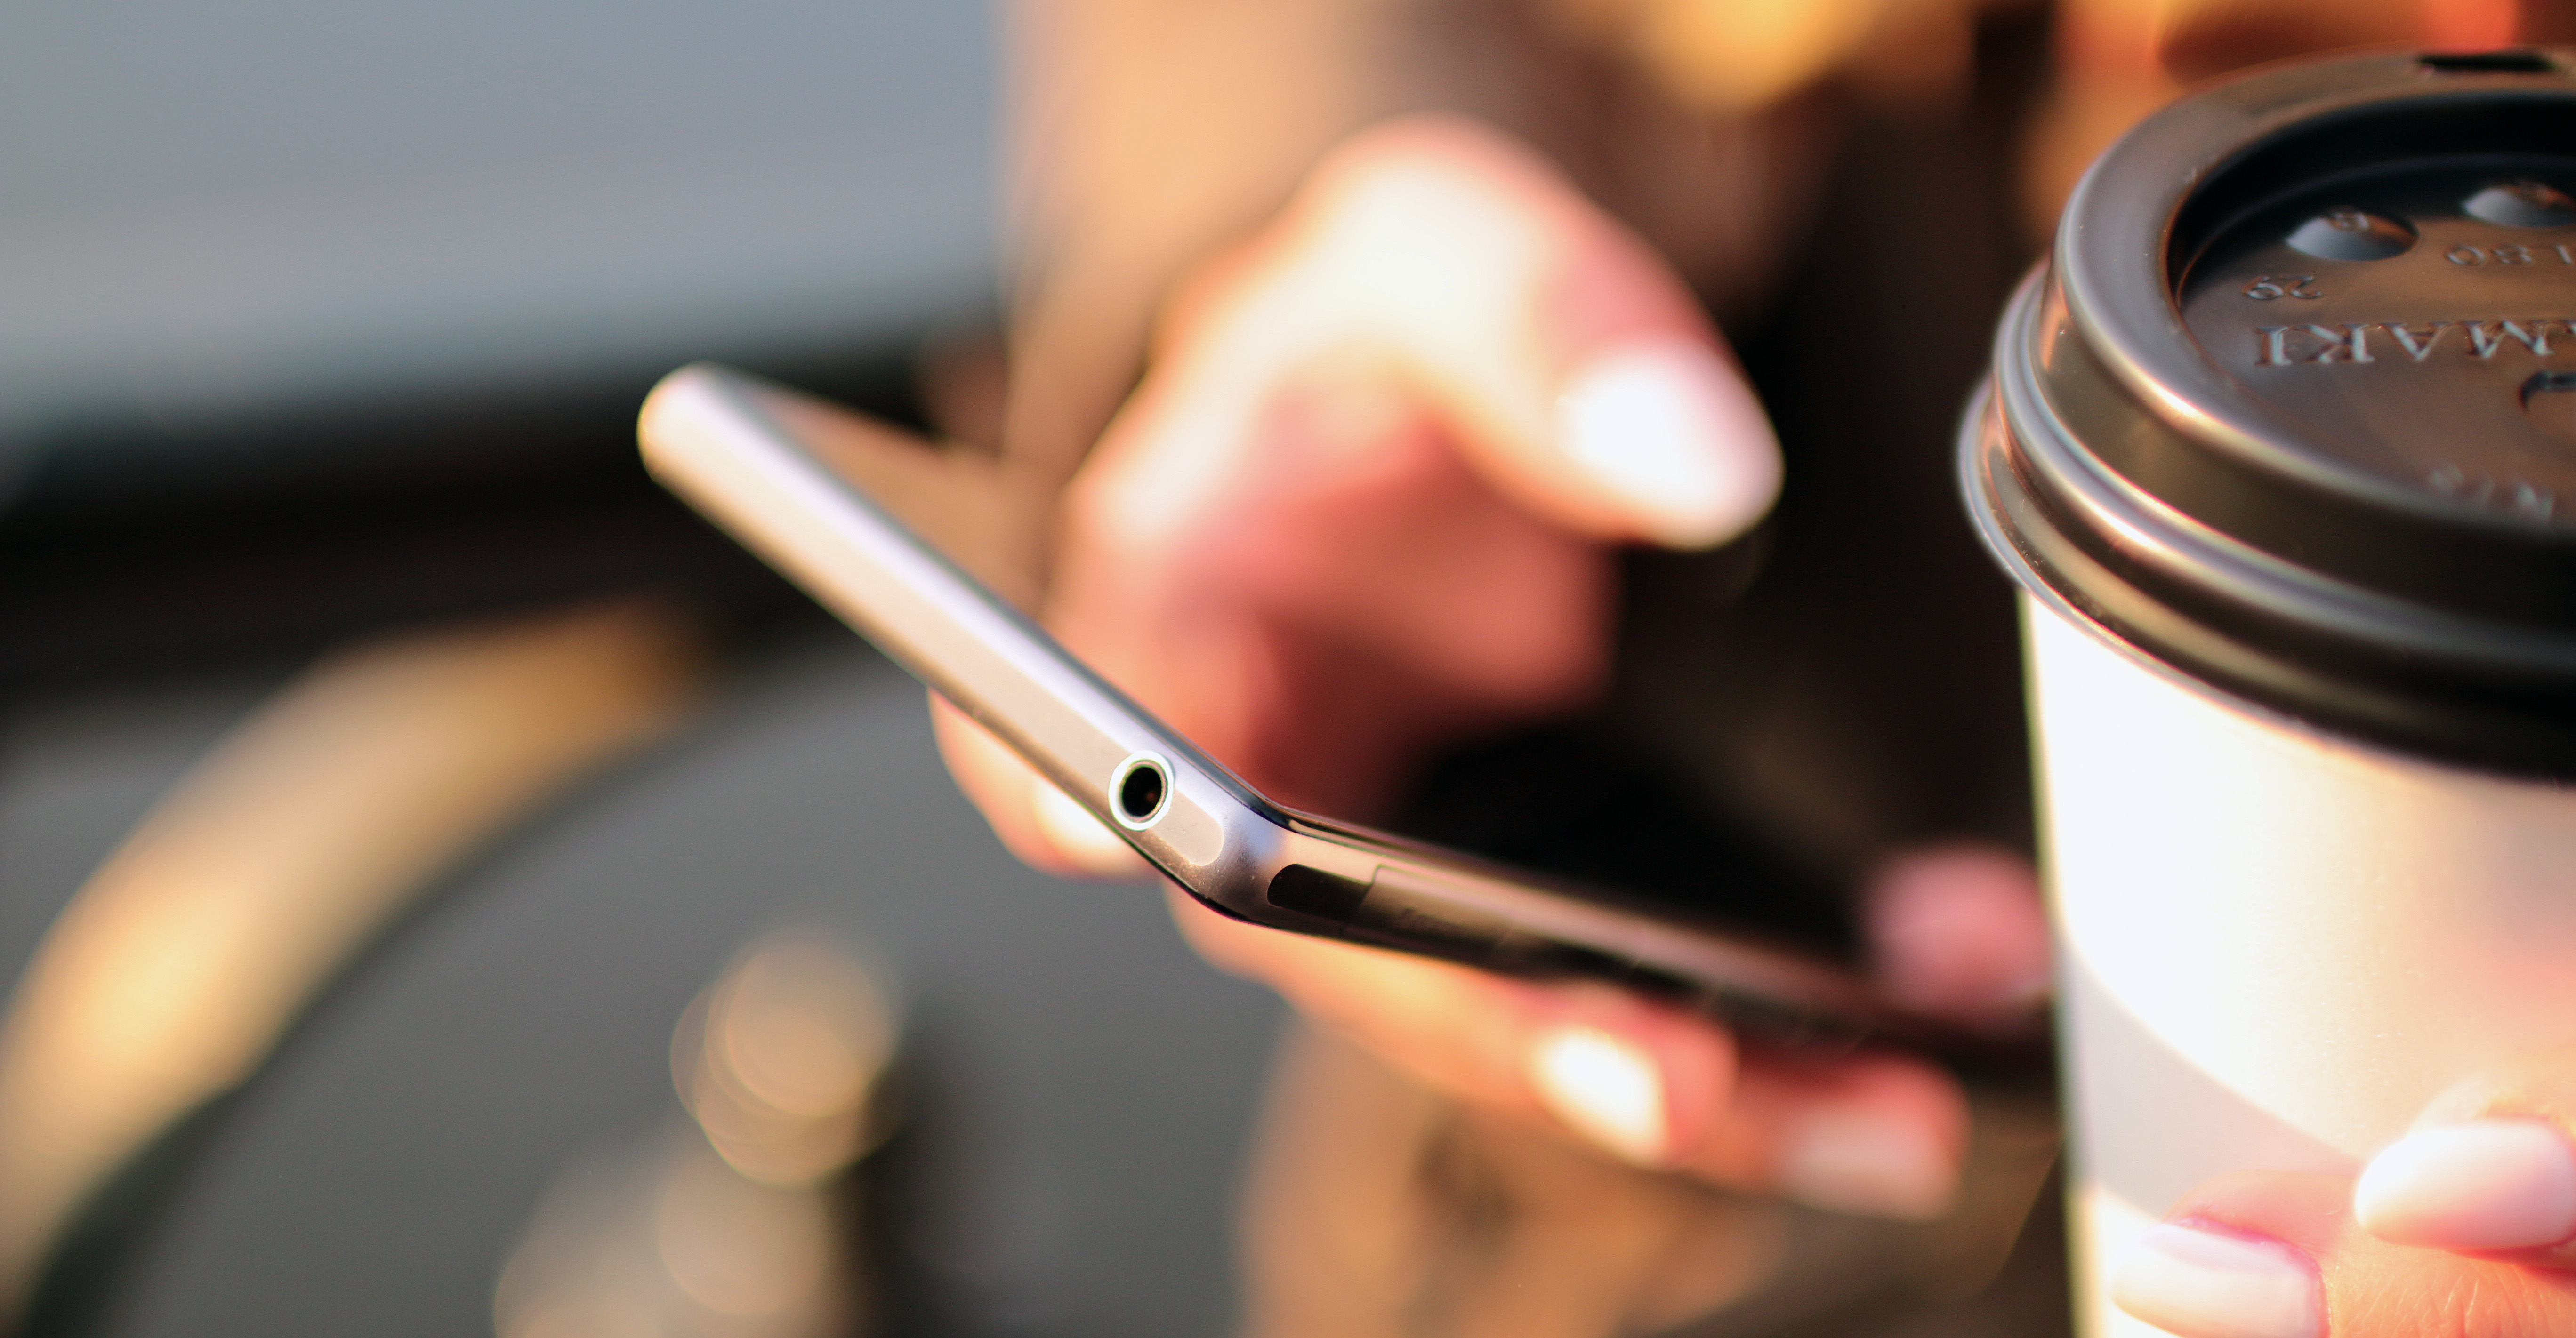
\includegraphics[width=1.5\textwidth]{Img/hands-coffee-smartphone-technology}
\end{center}
\caption{A hirer on the go}
\end{figure}

When a hirer is out on the go, perhaps traveling in a foreign city or commuting, Hire will provide contextual suggestions based on that context. This could be suggesting food delivery in the area or someone to grab you coffee as you drive between meetings.

\subsubsection{For Hirees}

When a hiree is at home, Hire will provide situational notifications of jobs in their area. The information made available to the hiree will be tailored based on schedule, previous experience, and interests. The hiree will have control over the these settings so they can be notified when a job appropriate for them is available.

When on the go, a hiree will have the option to be made aware of local jobs that relate to their skill sets. Hirees could also be made aware of possible tasks when during a trip or a commute at their discretion. For example a hiree could be notified of a food delivery on their ay home from work.

\subsection{Scenarios}

The following section details two example interactions between hirer or hirees and the Hire platform. The two scenarios are,

\begin{description}
    \item[Hiring from home] Sarah would like some help unclogging her shower drain which is full of hair.
%    \item[Hiring on the go] Tim would like to have some good food delivered to his hotel room while on a business trip.
%    \item[Getting hired from home] Justin gets notified about about a job helping a hirer down the street with yard work.
    \item[Getting hired on the go] Andy gets notified about a job to pick up a hirer's dry cleaning on his way home from work.
\end{description}

\subsubsection{Hiring from Home}

Sarah's roommate has complained about the shower not draining and now Sarah is tasked with cleaning out the drain. Sarah tries cleaning it with a drain snare but quickly realizes she doesn't have the stomach for it (see figure \ref{fig:sarahs-drain}).

\begin{figure*}[htb]
    \centering
    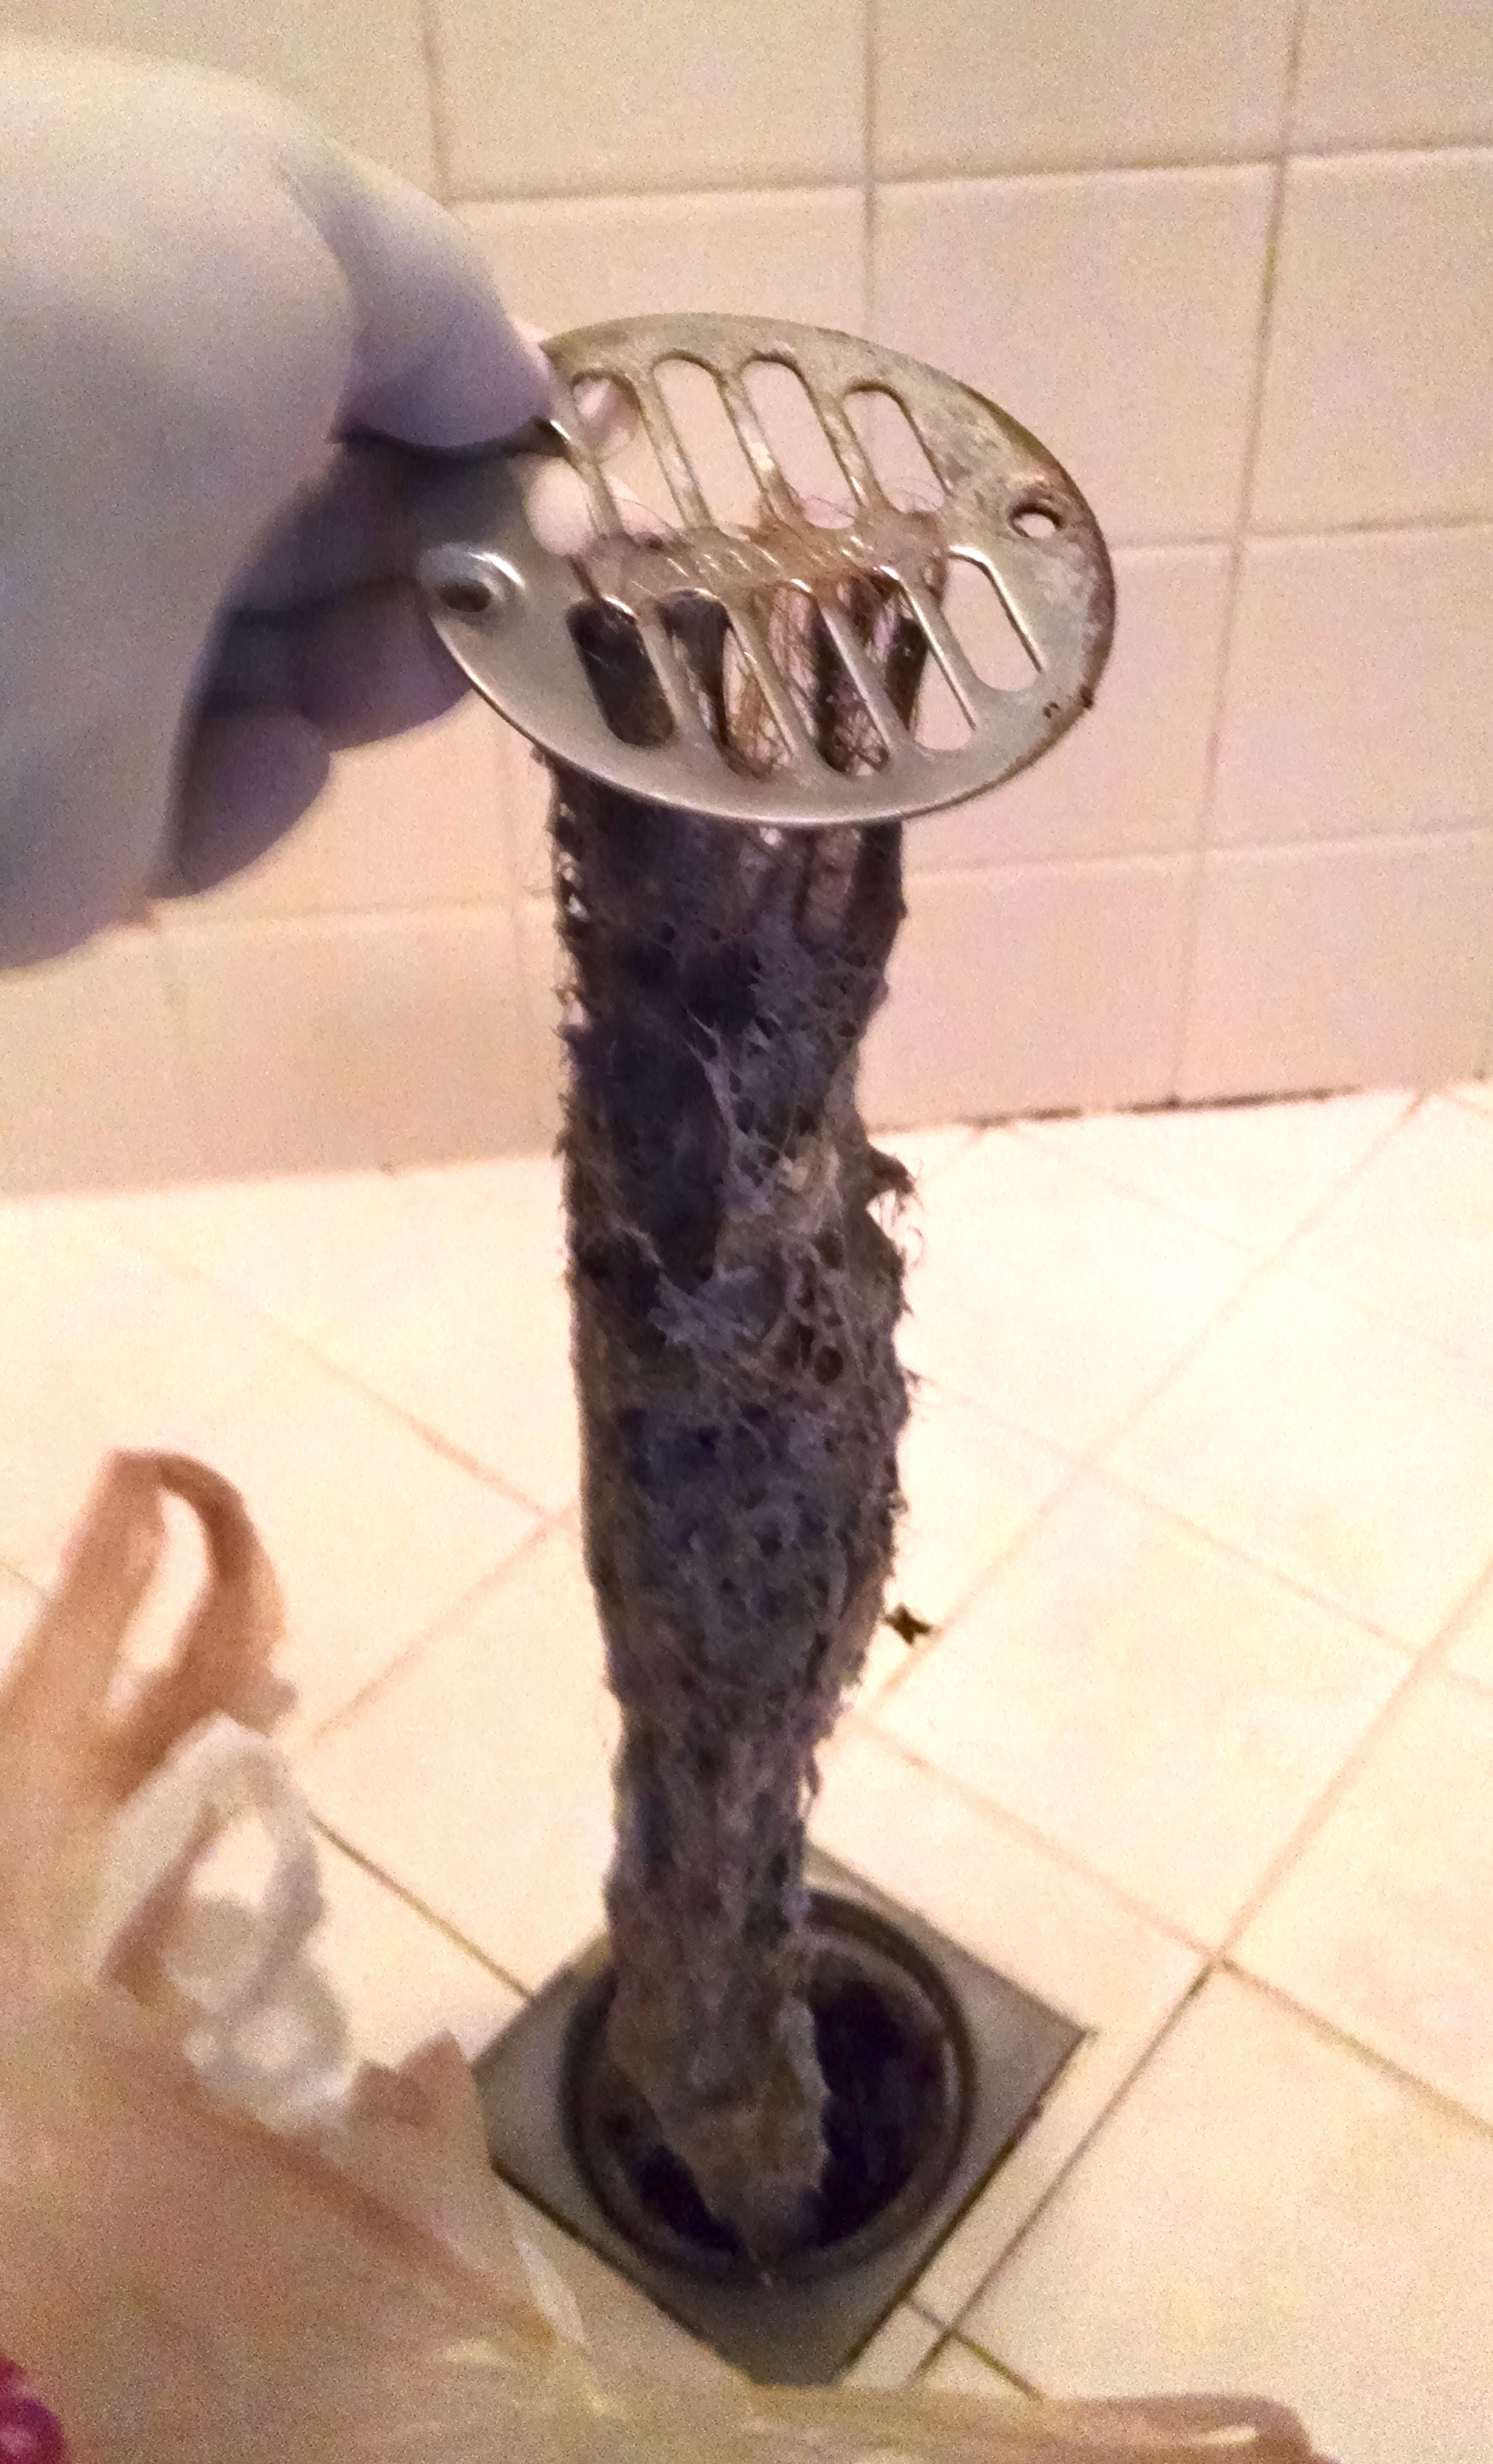
\includegraphics[width=0.5\textwidth]{Img/showerhair}
    \caption{The hair from Sarah's Drain}\label{fig:sarahs-drain}
\end{figure*} 

Sarah decides to contact someone for help. She grabs the Hire app from her devices app store. Being a first time user Sarah is prompted to sign up upon opening the app. She chooses to create an account using her Facebook account and the app pulls her details from Facebook. She is then prompted to add a credit card. The interface provides either the option to fill in credit card details or to read the details off her credit card using the camera. After choosing the latter Sarah is brought to the home screen where the on boarding wizard offers to help her create her first job. 

Sarah fills out the fields for job description, location (inferred by the app), offer amount, notes, and timeframe. Sarah's job is called "Clean out my shower drain", she gives it a timeframe of a couple hours and an offer amount of \$20. In the notes Sarah mentions that she already has a drain snare.

About twenty minutes after posting Sarah receives a notification that Joe, a hiree, has offered to do her job but for \$30. After reviewing Joe's hiring history and reviews, Sarah agrees and a hold is placed for the \$30 on her credit card. Joe sends a message through Hire to Sarah asking if she has any Draino before he comes over. Sarah responds that she does and sends Joe her address. 

Joe shows up a half hour later and gets started cleaning out the drain while Sarah watches TV in the other room. When Joe's done he marks the job done on his phone and logs a picture with the app. Sarah is notified and also marks it as done which transfers the funds to Joe's PayPal. Joe leaves and a little while later Sarah is prompted to fill out feedback for Joe, she gives him five stars for his prompt service and cheerful attitude.

\subsubsection{Getting Hired on the Go}

Andy has about an hour left at his work when he gets a notification from the Hire app. Someone nearby would like their dry cleaning picked up and delivered and it's on Andy's route home from work. The job is offering \$15 and, after opening the notification, Andy accepts. He sends a message to Dan, the Hirer, saying he will drop the dry cleaning off in about an hour when he's off work. Dan responds and sends Andy the confirmation number and address to pick up the dry cleaning.

Andy gets off work and drives to the dry cleaners. He picks up the clothes and heads to Dan's place. He arrives and gives Dan the dry cleaning. On the way back to his car, Andy marks the job as done. Several minutes later he's notified that Dan did as well and the funds are deposited into Andy's PayPal account. Andy is offered the chance to offer feedback for Dan and gives him five stars for being prompt and responsive.

A couple weeks later, once Andy has been hired by a few different hirers, he gets a summary of his feedback in his email. He sees that he received all good feedback. 

%
% MANAGEMENT PLAN
% ---------------------------------------
\section{Management Plan}\label{management-plan}
% ├── The management plan of about five pages should include a breakdown
% │   of the different features of the project, the major classes of
% │   functions and the relationship between them.
% ├── It should also include a page or so discussing possible
% │   implementations.
% ├── Make sure that you do not give the impression that you are
% │   promising more than you intend to deliver.
% ├── Cover yourself by including a page on a minimal system that you
% │   think you can complete by the end of term, and the enhancements
% │   you could include if all goes well.
% └── Finish with a summary restating the main points you want the
%     customer to remember, then include a page on the structure of your
%     team and who will be responsible for which parts of the project.

\subsection{Features}

% TODO: Features (Jake)

\subsection{Architecture}

% TODO: Architecture (Jake)

\subsection{Implementation}

Our technology stack will be organized into a \gls{client} \gls{server} model. Connections will be initiated through a \gls{frontend} (either \gls{android} or \gls{ios}) and requests will be handled by a \gls{server} written in \gls{scala} \cite{scala}. 

This \gls{server} will be securely hosted by \gls{digitalocean} and will be implemented with \gls{hscaling} as a top priority. This means that instead of moving our \gls{server} to a more powerful machine as we get more traffic, we will simply add more \glspl{server} and split the load between them.

The final piece will be handling monetary transactions, which will be completed using the \gls{paypal} \gls{rest} \gls{api} \cite{paypal}. Using a mature service like \gls{paypal} will ensure that monetary transactions are fast secure and simple.

%
% SUMMARY
% ---------------------------------------
\section{Summary}

% TODO: Summary (Jonah)

    
%%%%%%%%%%%%%%%%%%%%%%%%%%%%%%%%%%%%%%%%%%%%%%%%%%%%%%%%%%%%%%%%%%%%%%%%%%%%%%%
 
%    \pagebreak
    \section{References} 
    
    \bibliographystyle{IEEEtran}

    \bibliography{references}
    
    \pagebreak
%   ____             _      __  __       _   _            
%  | __ )  __ _  ___| | __ |  \/  | __ _| |_| |_ ___ _ __ 
%  |  _ \ / _` |/ __| |/ / | |\/| |/ _` | __| __/ _ \ '__|
%  | |_) | (_| | (__|   <  | |  | | (_| | |_| ||  __/ |   
%  |____/ \__,_|\___|_|\_\ |_|  |_|\__,_|\__|\__\___|_|   
%  

% Appendices

%\pdfbookmark[part]{Appendices}{appx}
%\begin{appendices}
%
%\section{Tool Screen Captures}\label{appx:screens}
%
%
%\end{appendices}

\end{document}
